\pgfplotstablegetelem{\thepart}{[index]\columnIndex}\of{\cronograma}
\part{\pgfplotsretval}
\label{part:\thepart}
\frame{\partpage}




\begin{frame}[t]{Padrões de desenvolvimento de software}
	
	\fontsize{12pt}{15.2}\selectfont{
		...continuando Padrões de desenvolvimento de software.\\ 
	}\par
	\vspace{1em}
	
	
	\fontsize{12pt}{15}\selectfont{
		\begin{itemize}%[<+->]  
			
			\item {\color{red}Padrões de Criação.}
			
				\begin{itemize}%[<+->]
					\item {\color{blue}Singleton \CheckmarkBold}
					\item Abstract Factory \XSolidBrush
					\item Builder \XSolidBrush
					\item Factory Method \XSolidBrush
					\item Prototype \XSolidBrush
				\end{itemize}
				
		\end{itemize}
	}\par
	\vspace{1em}
	
	
\end{frame}




\begin{frame}[t]{Padrões de criação}

	\fontsize{12pt}{15.2}\selectfont{
		Abstract Factory \CheckmarkBold

	}\par
	\vspace{1em}


	\fontsize{12pt}{15}\selectfont{
		\begin{itemize}%[<+->]  

			\item fornece uma interface para criar famílias de objetos relacionados ou dependentes sem especificar suas classes concretas.

			\item Em outras palavras, ele permite que você crie objetos sem precisar saber exatamente qual classe concreta será instanciada.

		\end{itemize}
	}\par
	\vspace{1em}

\end{frame}



\begin{frame}[t]{Padrões de criação - Abstract Factory}
	
	\fontsize{12pt}{15.2}\selectfont{
		Principais considerações:

	}\par
	\vspace{0.5em}


	\fontsize{12pt}{14}\selectfont{
		\begin{enumerate}%[<+->]
			
			\item \textbf{AbstractFactory}: Define uma interface para criar produtos abstratos. Normalmente, essa interface declara métodos para criar cada tipo de produto que a fábrica pode produzir.
			
			\item \textbf{ConcreteFactory}: Implementa a interface da fábrica abstrata e produz instâncias concretas dos produtos.
			
			\item \textbf{AbstractProduct}: Declara uma interface para um tipo de produto. Cada produto específico deve implementar essa interface.
			
			\item \textbf{ConcreteProduct}: Implementa a interface do produto abstrato. Cada fábrica concreta criará instâncias desse tipo de produto.
			
			\item \textbf{Client}: Usa apenas as interfaces definidas pela fábrica abstrata e pelos produtos abstratos para trabalhar com os objetos. O cliente não precisa saber quais classes concretas estão sendo usadas.
			
		\end{enumerate}
	}\par
	\vspace{1em}

\end{frame}







\begin{frame}[t]{Padrões de criação - Abstract Factory}
	
	\fontsize{14pt}{15.2}\selectfont{
		Tem por objetivo permitir a criação de famílias de objetos relacionados sem depender de suas classes concretas. Em Python, esse padrão é frequentemente usado para fornecer uma \textit{interface} para criar objetos em uma \textbf{superclasse}, enquanto permite que \textbf{subclasses} alterem o tipo de objetos que serão criados.
		
	}\par
	\vspace{0.5em}
	
	
	\fontsize{16pt}{15}\selectfont{
		\begin{enumerate}%[<+->]
			
			\item Define uma interface para criar objetos, mas não implementa os métodos de criação.
			
			\item Subclasses específicas (concretas) implementam a criação dos objetos, fornecendo diferentes implementações de uma família de objetos relacionados.
			
		\end{enumerate}
	}\par
	\vspace{1em}
	
\end{frame}




\begin{frame}[t]{Padrão de projeto Abstract Factory}
	
	\lstinputlisting[style=CBruno,caption=Código da Classe Cadeira Abstrata]{outros/codigos/python/exemplos-de-aulas/src/codigo_015_cadeira_abstrata.py}

	\lstinputlisting[style=CBruno,caption=Código da Classe Sofa Abstrato]{outros/codigos/python/exemplos-de-aulas/src/codigo_015_sofa_abstrato.py}

\end{frame}


\begin{frame}[t]{Padrão de projeto Abstract Factory}
	
	\lstinputlisting[style=CBruno,caption=Código da Classe Cadeira Concreta]{outros/codigos/python/exemplos-de-aulas/src/codigo_015_cadeira_classica_concreta.py}
	
	\lstinputlisting[style=CBruno,caption=Código da Classe Sofa Concreta]{outros/codigos/python/exemplos-de-aulas/src/codigo_015_sofa_classico_concreta.py}
	
\end{frame}



\begin{frame}[t]{Padrão de projeto Abstract Factory}
	
	\lstinputlisting[style=CBruno,caption=Código da Classe Cadeira Moderna]{outros/codigos/python/exemplos-de-aulas/src/codigo_015_cadeira_moderna_concreta.py}
	
	\lstinputlisting[style=CBruno,caption=Código da Classe Sofa Moderna]{outros/codigos/python/exemplos-de-aulas/src/codigo_015_sofa_moderno_concreta.py}
	
\end{frame}



\begin{frame}[t]{Padrão de projeto Abstract Factory}
	
	\lstinputlisting[style=CBruno,caption=Código da Classe Moveis Factory Abstrato]{outros/codigos/python/exemplos-de-aulas/src/codigo_015_moveis_factory_abstrato.py}
	
\end{frame}


\begin{frame}[t]{Padrão de projeto Abstract Factory}

	\lstinputlisting[style=CBruno,caption=Código da Classe Cadeira Classica Factory Concretra]{outros/codigos/python/exemplos-de-aulas/src/codigo_015_moveis_classicos_factory_concreto.py}
	
	\lstinputlisting[style=CBruno,caption=Código da Classe Sofa Classica Factory Concretra]{outros/codigos/python/exemplos-de-aulas/src/codigo_015_moveis_modernos_factory_concreto.py}

\end{frame}



\begin{frame}[t]{Padrão de projeto Abstract Factory}

	\lstinputlisting[style=CBruno,caption=Código da função código do cliente]{outros/codigos/python/exemplos-de-aulas/src/codigo_015_codigo_cliente.py}

\end{frame}




\begin{frame}[t]{Pytest}
	
	\vspace{-0.5em}
	\lstinputlisting[style=CBruno,caption=Cobertura de testes da função codigo cliente]{outros/codigos/python/exemplos-de-aulas/tests/test_codigo_015_cliente.py}
	
\end{frame}





\begin{frame}[t]{Padrões de criação - Abstract Factory}
	
	\fontsize{14pt}{15.2}\selectfont{
		Resumo
		
	}\par
	\vspace{0.5em}
	
	
	\fontsize{16pt}{15}\selectfont{
		\begin{enumerate}%[<+->]
			
			\item O padrão Abstract Factory permite a criação de famílias de objetos relacionados (por exemplo, móveis modernos ou classicos) sem especificar as classes concretas que os compõem.
			
			\item Isso promove a flexibilidade e extensibilidade no código, já que novas famílias de objetos podem ser introduzidas sem modificar o código existente.
			
		\end{enumerate}
	}\par
	\vspace{1em}
	
\end{frame}



\begin{frame}[t]{Abstract Factory}
	\vspace{1em}
	\centering
	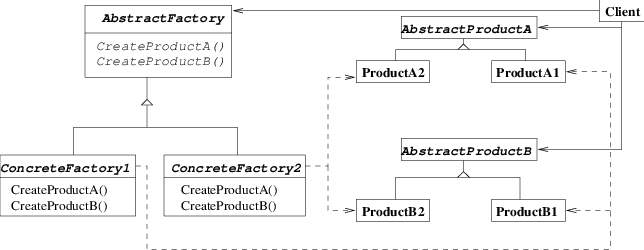
\includegraphics[scale=0.95]{imagens/fig-abstract-factory-diagram.png}

\end{frame}


\begin{frame}[t]{Exercícios}
	
	\fontsize{12pt}{19}\selectfont{
		Escreva o algoritmo e programa. Use \gls{poo} para resolver.
		\begin{itemize}%[<+->]
			
			\item \glsfirst{exercicio_029}: \glsdesc{exercicio_029}
			
			\vspace{1em}
			\centering
			
\includegraphics[scale=0.15]{imagens/fig-atencao-pessoas-estudando.png}
			
		\end{itemize}
	}\par
	\vspace{1em}
	
\end{frame}






